After creation of the class \texttt{Root} in section
\ref{sec:dispatcherTemplate} where we easily can
add new Generators and the defintion of the
\texttt{JsfOutputConfigurationProvider} in section \ref{sec:outputConfigurationProvider}
which prvides an output folder for JSF
artifacts, we use the \emph{New Xtend Class Wizard} to create a new Xtend class
called \texttt{JSFGenerator.xtend} in package \texttt{org.eclipse.xtext.example.ql.generator}.

This class will be our entry point to generate JSF related artifacts. The
\emph{New Xtend Class Wizard} provides the possibility to bind interfaces to the
new class by use of the \texttt{Add} button near the interface section.

\begin{center}
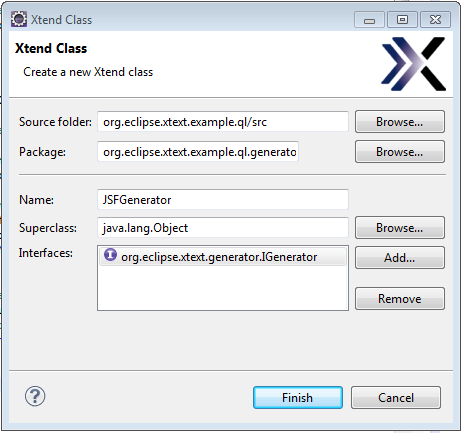
\includegraphics[width=8cm]{./images/chapter02/newXtendClassWizard.png}
\end{center}

As we want to create a new generator we add the interface
\texttt{org.eclipse.xtext.generator.IGenerator} to our new Xtend class.
After typing in the package, the name and the interface of our new Xtend class
as shown in the figure above, we can finish the
wizard so that the class shown in the following listing
will be created in our project.

\begin{lstlisting}[language=Xtend] 
package org.eclipse.xtext.example.ql.generator

import org.eclipse.xtext.generator.IGenerator
import org.eclipse.emf.ecore.resource.Resource
import org.eclipse.xtext.generator.IFileSystemAccess

class JSFGenerator implements IGenerator {
	
	override doGenerate(Resource input, IFileSystemAccess fsa) {
		throw new UnsupportedOperationException("TODO: auto-generated method stub")
	}
}
\end{lstlisting}

To get the created \texttt{JSFGenarator} executed we have to inject and dispatch
to it in our dispatcher template \texttt{Root.java} which was created in section
\ref{sec:dispatcherTemplate} earlier.

\begin{lstlisting}[language=Java] 
 package org.eclipse.xtext.example.ql.generator;

import javax.inject.Inject;

import org.eclipse.emf.ecore.resource.Resource;
import org.eclipse.xtext.generator.IFileSystemAccess;
import org.eclipse.xtext.generator.IGenerator;
import org.eclipse.xtext.xbase.compiler.JvmModelGenerator;

public class Root implements IGenerator {
  @Inject
  JvmModelGenerator jvmModelGenerator;
  @Inject
  JSFGenerator jsfGenerator;

  public void doGenerate(Resource input, IFileSystemAccess fsa) {
    // dispatch to other generators
    jvmModelGenerator.doGenerate(input, fsa);
    jsfGenerator.doGenerate(input, fsa);
  } 
}
\end{lstlisting}

Now it is time to add some functionality to the \texttt{JSFGenarator}. Open the
file \texttt{JSFGenarator.xtend} and go to the \texttt{doGenerate} extension
which is responsible to generate artifacts. Delete the auto-generated body of
the extension - initially it just throws an
\texttt{UnsupportedOperationException} - and add the following lines as first
statements to prevent execution of the generator if the file extension does not fit.

\begin{lstlisting}[language=Java] 
  if (input.URI.fileExtension!="ql")
            return
\end{lstlisting}

After this pre condition is passed we want to execute the generator logic for
our model so it is a good idea to save the models root node in a variable.

\begin{lstlisting}[language=Java] 
  val questionnaire = input.contents.head as Questionnaire 
\end{lstlisting}

Because we want to generate JSF artifacts into the \texttt{WebContent} folder
in the following steps we let Guice add a \texttt{JSFOutputConfigurationProvider}
extension to our \texttt{JSFGenerator}.

\begin{lstlisting}[language=Java] 
class JSFGenerator implements IGenerator{
  @Inject extension JSFOutputConfigurationProvider
  ...
 }
\end{lstlisting}

After this we have the possibility to use the \texttt{WEB\_CONTENT} outlet
constant as described in section \ref{sec:outputConfigurationProvider}.\newline
The following paragraphs will describe the different extensions of the JSFGenerator
which are responsible to generate the JSF artifacts described in
\ref{subsec:referenceImpl}. In a real world project it can be a good decision to
seperate different artifacts in different \texttt{Xtend} files. Our sample is a
very simple one, so we will add a new extension definition derived from the
sample below to the \texttt{JSFGenerator.xtend} class which encapsulates the
logic to generate a single artifact.

\begin{lstlisting}[language=HTML] 
  def generate_Artifact (EObject modelInfo)
  '''<?xml version='1.0' encoding='UTF-8' ?>
      <!-- @generated -->
      <!DOCTYPE html PUBLIC "-//W3C//DTD XHTML 1.0 Transitional//EN" "http://www.w3.org/TR/xhtml1/DTD/xhtml1-transitional.dtd">
      <html xmlns="http://www.w3.org/1999/xhtml"
        xmlns:h="http://java.sun.com/jsf/html"
        xmlns:ui="http://java.sun.com/jsf/facelets">
     ...
      </html>
  '''
\end{lstlisting}

To get a valid xhtml page we have to generate the DOCTYPE
and HTML tag into each xhtml file what was replaced in the following
listings to focus on what matters.